\vspace{30px}\section{Background}
This chapter focuses on a brief explanation of the physics behind thermistors by introducing and discussing the structure of the atom and the most crucial information that is needed for a better understanding of the topic. Then the attention will be shifted to discussing a specific type of material, known as semiconductors, that are largely utilized for the creation of electric components as far as thermistors.
\todo{Finish Background introduction}


\subsection{Outermost orbit and valence electrons}
As is common knowledge, everything is made out of atoms, every living creature and every unanimated object. An atom is made out of three subatomic particles. The protons (which have a positive electric charge) and the neutrons constitute the nuclei of the atom. The electrons, carrying a negative charge, orbit around the nucleus in distinct orbits.

By observing the figure \ref{fig:atom-structure}, it is possible to distinguish two important types of electrons: the inner electrons, which orbit around the inner shells, and the valence electrons that orbit in the \textbf{valence shell} (also called the outermost orbit). These electrons are crucial for determining the properties of the material \cite{Gupta20163}.
\begin{figure}[h]
    \centering
    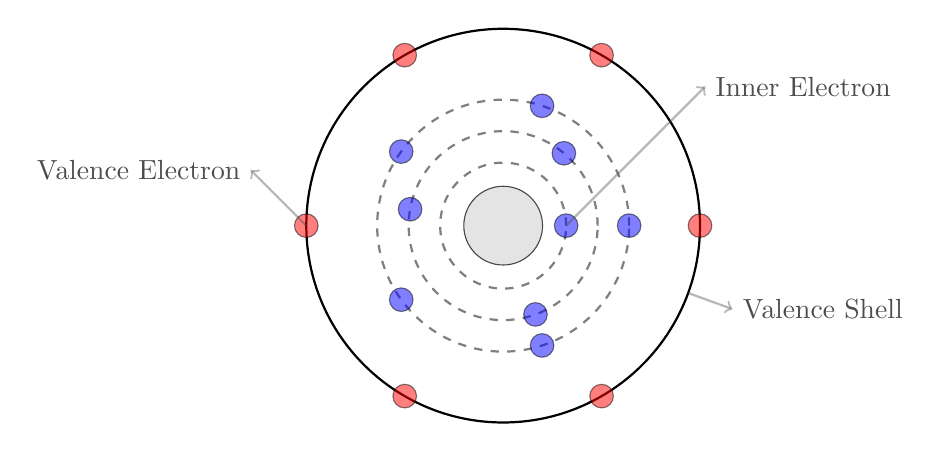
\begin{tikzpicture}[scale=1]

  % Atom nucleus
  \draw[fill=gray!30, opacity=0.7] (0,0) circle (0.5);
  
  % 1st orbit
  \draw[thick, dashed, opacity=0.5] (0,0) circle (0.8);
  \draw[fill=blue, opacity=0.5] (0:0.8) circle (0.15);
  
  % 2nd orbit
  \draw[thick, dashed, opacity=0.5] (0,0) circle (1.2);
  \foreach \angle in {50,170,290}
    \draw[fill=blue, opacity=0.5] (\angle:1.2) circle (0.15);
  
  % 3rd orbit
  \draw[thick, dashed, opacity=0.5] (0,0) circle (1.6);
  \foreach \angle in {72, 144, 216, 288, 360}
    \draw[fill=blue, opacity=0.5] (\angle:1.6) circle (0.15);
  
  % Valence shell (4th orbit)
  \draw[thick] (0,0) circle (2.5);
  \foreach \angle in {60, 120, 180, 240, 300, 360}
    \draw[fill=red, opacity=0.5] (\angle:2.5) circle (0.15);
  
  % Arrow pointing out one inner electron (longer)
  \draw[->, thick, black!70, opacity=0.4] (0:0.8) -- ++(45:2.5) node[right, text opacity=1] {Inner Electron};
  
  % Arrow pointing out one valence electron
  \draw[->, thick, black!70, opacity=0.4] (180:2.5) -- ++(135:1) node[left, text opacity=1] {Valence Electron};
  
  % Arrows describing the outermost orbit
  \draw[->, thick, black!70, opacity=0.4] (340:2.5) -- ++(340:0.6) node[right, text opacity=1] {Valence Shell};
  
  \end{tikzpicture}
  
    \caption{The orbits and electrons of an atom.}
    \label{fig:atom-structure}
\end{figure}
Particularly depending on how much energy these electrons have, a material is going to be a good conductor rather than a good insulator.

When the outermost orbit is incomplete, valence electrons are separable from the atom. In some cases, at room temperature, there is enough energy to remove these electrons from the orbit. This is the case for most conductive elements like metals (copper, silver and gold) which can easily propagate both electricity and heat. On the other hand, when a great amount of energy is needed to remove one valence electron from the valence orbit, the material is an insulator (also known as dielectric) like wood, glass or rubber \cite{Gupta20163}. 

\subsection{Semiconductor materials}
Other than conductors and dielectric elements there are other types of materials like semiconductors. This particular type of material is rather important to discuss because it is the key element in creating a thermistor. The peculiarity of a semiconductor element is that its conductivity stands between the inductors and the dielectric materials. The most common semiconductor materials are silicon and germanium but it is also used zinc, cadmium, boron and more \cite{Gupta20163}. These types of materials are highly popular because of their properties:
\vspace{-3px}\begin{itemize}
\renewcommand*{\labelitemi}{$\circ$}
\setlength{\itemsep}{-2px}
    \item They are light weight-wise and small dimension-wise;
    \item They are highly energy-efficient because they work with low voltage;
    \item Long-term degradation effects are insignificant.
\end{itemize}

\noindent Additionally, generally, the semiconductor materials are \textsl{negative temperature coefficient} meaning that their conductivity increases with the temperature, and so the resistivity of the element decreases non-linearly. But this also means that when the temperatures are extremely low (near zero Kelvin) their conductivity properties are comparable to a dielectric material (so their resistance is extremely high).

It is important to note that the semiconductors do not follow Ohm's law. More precisely the current increases much more than the voltage; this peculiarity is used for the BJT transistors. Furthermore, specifically because of the resistivity/temperature curve they are widely used in thermistors, rectifiers, Zener diodes, varistors and photovoltaic cells \cite{Gupta20163}.


\subsubsection*{Other types of materials}
It is worth mentioning that the three types of material aforementioned are not the only ones. The \textsl{superconductors} are materials whose electrical resistivity reaches almost zero when the temperature is greatly below zero Celsius. These materials are usually metals or ceramics \cite{Gupta20163}.

Moreover, there are \textsl{magnetic materials} that can differ in several types depending on their capability of being magnetized by magnetic fields. The diamagnetic and paramagnetic materials have a very low magnetic susceptibility (between $10^{-6}$ and $10^{-3}$) meaning that they are not likely to propagate a magnetic field. Then there are the ferromagnetic and ferrimagnetic materials whose magnetic susceptibility depends on the magnetic field strength. Eventually, there are also antiferromagnetic materials whose susceptibility increases as the temperature increases but when the element reaches a critical temperature, the susceptibility starts decreasing again \cite{Gupta20163}\cite{heck2013magnetic}.

Furthermore, it is also important to mention the \textsl{ferroelectrics} which are a type of material whose natural electric polarization can be changed by the presence of an electric field \cite{Gupta20163}\cite{whatmore2017ferroelectric}.

\subsection{History of thermistors}
\cite{Feteira2009967}
\todo{Insert history of thermistor}
